% ============================================================
%  CHAPTER 1: INTRODUCTION
% ============================================================

\chapter{INTRODUCTION}
\label{chap:introduction}

\section{Background and Motivation}
\label{sec:vpn_background}

A Virtual Private Network (VPN) is an indispensable network security technology designed to establish an encrypted communications tunnel across untrusted public intermediate networks, such as the global Internet~\cite{stallings2022cryptography}. When an application on a client device issues outbound network traffic, the operating system routes raw Layer~3 Internet Protocol (IP) datagrams to a specialized virtual network interface (TUN driver in Linux~\cite{huelsing2022pqwireguard}, or \texttt{android.net.VpnService} in Android~\cite{android_vpnservice_docs}). The tunneling software encrypts these datagrams using symmetric cryptography, wraps them in transport framing, and dispatches them to a remote security gateway that decrypts and routes them to their final destination~\cite{rfc9370}.

However, mainstream contemporary VPN architectures (OpenVPN, IPsec, WireGuard) rely exclusively on classical asymmetric cryptographic primitives---such as RSA, Diffie-Hellman (DH), and Elliptic Curve Diffie-Hellman (ECDH/X25519)---for key exchange and digital authentication~\cite{alagic2022nist,huelsing2022pqwireguard}. These mathematical problems rely on integer factorization and discrete logarithms, which can be solved in polynomial time by a sufficiently powerful Cryptographically Relevant Quantum Computer (CRQC) executing Shor's algorithm~\cite{mavroeidis2022impact}.

\begin{figure}[htbp]
  \centering
  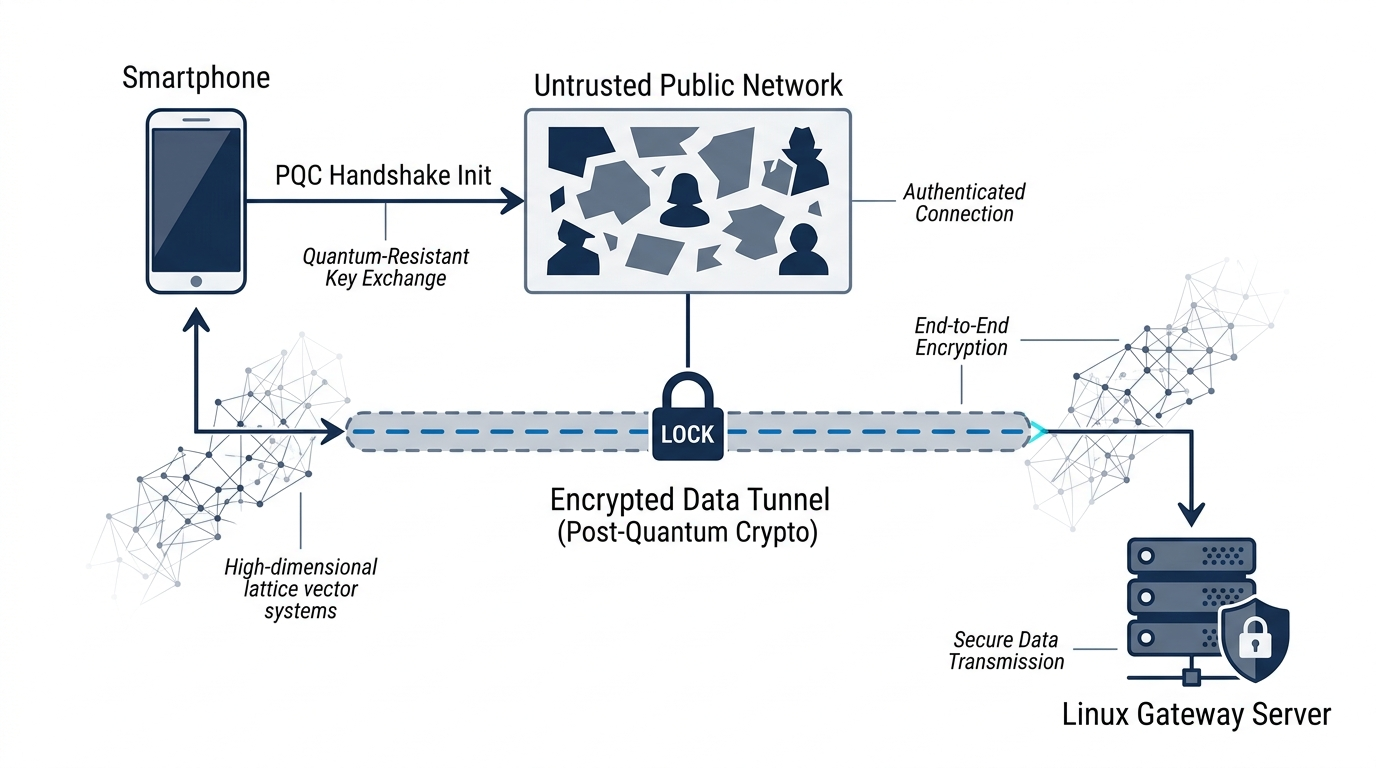
\includegraphics[width=0.88\linewidth,height=0.32\textheight,keepaspectratio]{figures/vpn_cover_graphic.jpg}
  \caption[Conceptual Architecture of Mobile VPN Tunneling]{Conceptual Architecture of Mobile VPN Tunneling: This figure illustrates the end-to-end tunneling of Layer~3 IP datagrams across untrusted transit carriers to the secure gateway.}
  \label{fig:vpn_cover_overview}
\end{figure}

The threat is not merely futuristic. Under the ``Harvest Now, Decrypt Later'' (HNDL) doctrine, adversaries and intelligence organizations routinely intercept and store encrypted network traffic traversing global transit backbones today. Once large-scale quantum computers materialize, adversaries will retroactively decrypt this archived ciphertext. In accordance with Mosca's Theorem of Quantum Risk~\cite{joseph2022transitioning,mosca2023threat}, if the shelf-life of secret data ($x$) plus the migration timeline to quantum-safe algorithms ($y$) exceeds the arrival time of a quantum computer ($z$), security is already breached ($x + y > z$). Therefore, migrating mobile communications to Post-Quantum Cryptography (PQC) is an immediate engineering mandate.

\section{Problem Statement and Objectives}
\label{sec:problem_statement}
\label{sec:project_objectives}

Existing VPN implementations on Android present severe security and architectural limitations:
\begin{enumerate}[label=(\roman*)]
    \item Quantum Vulnerability: Standard Android VPN clients deploy classical key exchanges that offer zero resistance against quantum adversaries.
    \item Protocol Inefficiency on Mobile: Academic PQC prototypes developed in user space on Linux do not address mobile OS constraints, such as Android socket protection, Low Memory Killer (LMK) cycles, and battery-efficient multithreading.
    \item Cluttered Mobile Interfaces: Existing enterprise VPN applications exhibit complex, unintuitive user interfaces lacking real-time cryptographic telemetry.
\end{enumerate}

To resolve these challenges, this project formulates the following primary objectives:
\begin{enumerate}
    \item Post-Quantum Protocol Design: Engineer a lightweight, authenticated network tunneling protocol based on finalized NIST standards: ML-KEM-1024 (FIPS 203) for key encapsulation and ML-DSA-65 (FIPS 204) for gateway identity authentication~\cite{nist_fips_203,nist_fips_204}.
    \item Native Android Integration: Develop a robust Android client utilizing \texttt{android.\allowbreak net.\allowbreak VpnService}, enforcing kernel socket protection (\texttt{protect()}) to prevent feedback routing loops, and implementing non-blocking asynchronous packet I/O.
    \item Minimalist Declarative UI: Implement a modern, minimalist white-themed interface adhering to Google Material Design 3 and WCAG 2.1 accessibility guidelines, providing real-time cryptographic metrics.
    \item Gateway Implementation and Empirical Validation: Construct a hardened Linux gateway supporting dynamic IP address allocation, kernel packet forwarding, and hardware-accelerated AES-256-GCM symmetric encryption with 64-bit sliding-window anti-replay defenses.
\end{enumerate}

\section{Scope, Contributions, and Report Organization}
\label{sec:scope_contributions}

The primary technical contributions delivered by this project include:
\begin{itemize}
    \item Cryptographic Hybrid Pipeline: An end-to-end implementation coupling NIST FIPS 203 ML-KEM-1024 with HKDF-SHA256 (RFC 5869) and AES-256-GCM (NIST SP 800-38D).
    \item Native Android VpnService Pipeline: A production-grade Kotlin MVVM mobile application providing seamless capture and routing of system-wide IP packets.
    \item Linux Gateway with Automated NAT: A Python server daemon operating over virtual TUN interfaces (`tun0`) with dynamic IP pooling and `iptables` masquerading.
    \item Comprehensive Security and Performance Evaluation: Exhaustive empirical testing verifying packet integrity under active bit-flipping attacks, replay injection, and mobile throughput benchmarking.
\end{itemize}

The remainder of this report is organized into six core chapters as follows: Chapter~\ref{chap:literature_review} provides a comprehensive literature review and problem background, analyzing classical cryptosystem vulnerabilities, NIST standardization, Android socket architecture, and operational system requirements. Chapter~\ref{chap:system_design} formalizes system design and architecture, covering wire framing, cryptographic handshake sequencing, mathematical security proofs, pure-Kotlin Keccak alignment, and mobile UI architecture. Chapter~\ref{chap:implementation} details end-to-end implementation, including the Android VpnService lifecycle, Kotlin PQC engine, Python gateway daemon, and production deployment scripts. Chapter~\ref{chap:testing} presents exhaustive evaluation and security testing across unit verification, wire interoperability, adversary injection, Wireshark packet captures, and performance benchmarking. Chapter~\ref{chap:conclusion} concludes with project retrospectives, defensive strategies, lessons learned, and future enhancements.
